\section{Общая топология}
Раньше были телевизоры с \textit{бесконченым} количеством пикселей (это зависит от химических свойств вещества кинескоп).
\begin{center}
    \includegraphics[scale=0.8]{img/topology_tv_example}
\end{center}

\begin{definition}
    Топологическим пространством называется упорядоченная пара $(X, \Omega)$, $\Omega \subset 2^X$, причем выполнено 
    \begin{enumerate}
        \item $\emptyset, X \in \Omega$
        \item $\bigcup A_i \in \Omega$ если $\forall i\ A_i \in \Omega$
        \item $\bigcap_{n} A_i \in \Omega$, если $\forall i\ A_i \in \Omega$
    \end{enumerate}
\end{definition}

\begin{definition}
    Замкнутым называется множество $B$ такое, что его дополнение $X \setminus B \in \Omega$ открыто.
    \end{definition}

\begin{definition}
    Связным топологическим пространством называется такое топ. пространство $(X, \Omega)$, в котором нет $A,B \in \Omega$ таких, что $A \cup B = X$ и $A \cap B = \emptyset$.
\end{definition}

\begin{definition}
    Подпространством пространства $(X, \Omega)$ называется топологическое пространство $(X_1, \Omega_1)$, где $X_1 \subset X$ и $\Omega_1 =\{A \cap X_1 \mid A \in \Omega \}$.
    Это подпр-во так же называется индуцированным подпространством.
\end{definition}

Например, промежуток $[0, \frac{1}{2})$ не является открытым в $\mathbb{R}$, но является открытым в подпространстве, индуцированным $[0, 1]$.

\begin{definition}
    Подмножество пр-ва называется связным, если связно индуцированное им подпространство.
\end{definition}

Пример: множество $[0,1] \cup [2,3]$ является несвязным подмножеством $\mathbb{R}$. 

\begin{example}
    Определим топологию на ацикличном графе следующим образом: 
    подвесим все его деревья (компоненты связности) и назовём множество открытым, если вместе с каждой своей вершиной оно содержит его поддерево.      
\end{example}

\begin{theorem}
    Лес (ацикличный граф) связен титт., когда он связен как топ. пространство.
\end{theorem}

\section{Решетки}
\begin{definition}
    Рассмотрим частично-упорядоченное множество $X$, $(X, \leqslant)$.
    
    Множество верхних граней $\{a,b\}$~--- $\{ x \in X \mid a \leqslant x,\ b \leqslant x\}$.  
    
    Множество нижних граней $\{a,b\}$~$\{x \in X \mid a \geqslant x, b \geqslant x\}$.
    
    Наименьший элемент $A$~--- такой $a \in A$, что нет $b \in A$, такого что $b \leqslant a$.
    Аналогичное определение даётся наибольшему элементу.

    $a+b$~--- наименьший элемент множества верхних граней $\{a,b\}$.

    $a \cdot b$~--- наибольший элемент множества нижних граней $\{a,b\}$.

    $(X, \leqslant)$ называется решеткой, если для любых $a,b\in X$ определены $a+b$ и  $a\cdot b$.
\end{definition}

\begin{remark}
    Наибольший и максимум это не одно и то же!
\end{remark}

\begin{example}
    Топологическое пространство с порядком по включению является решеткой.
    
    Антипример: произвольное дерево не является решеткой.    
\end{example}

\begin{definition}
    Дистрибутивной решеткой называется такая решетка, в которой 
    \[(a+b)c = ac + bc \quad a + bc = (ab)+(ac)  \] 
\end{definition}

\begin{lemma}
    Для дистрибутивной решетки так же верно, что $a \cdot (b + c) = (a \cdot b) + (a \cdot c)$.
\end{lemma}

\begin{definition}
    Псевдодополнение $a\to b$ это наибольший $c$ из всех таких $c$, что $ac \leqslant b$.

    Решетка, в которой псевдодополнение определено для всех пар элементов, называется импликативной.
\end{definition}

\begin{figure}
    \begin{center}
        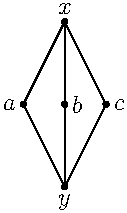
\includegraphics{img/diamont.pdf}
        \caption{Решетка, в которой для $a,b$ не определено псевдодополнение}
    \end{center}
\end{figure}

\begin{definition}
Ноль $0$ и единица $1$~--- это нейтральные элементы операций $+$ и $\cdot$ одновременно.     
Другими словами 
\begin{itemize}
    \item $0$~--- такой элемент, что $0 \leqslant x $ для всех $x$;
    \item $1$~--- такой элемент, что $x \leqslant 1 $ для всех $x$.
\end{itemize}
\end{definition}

% \begin{theorem}
%     Рассмотрим импилкативную решетку $(X, \leqslant)$ с 0.
%     Рассмотрим интуиционисткое исчисление высказываний, определим оценку следующим образом: 
%     $\llbracket \alpha \land \beta \rrbracket = \llbracket \alpha \rrbracket \cdot \llbracket \beta \rrbracket$, $\llbracket \alpha \lor \beta \rrbracket = \llbracket \alpha \rrbracket + \llbracket \beta \rrbracket$, $\llbracket \alpha \to \beta \rrbracket = \llbracket \alpha \rrbracket \to \llbracket \beta \rrbracket$, $\llbracket \neg \alpha \rrbracket = \llbracket \alpha \rrbracket \to 0$.
% \end{theorem}

\begin{theorem}
    Рассмотрим $\langle X, \Omega \rangle$~--- импликативную решетку с $0$. 
    % Рассмотрим И.И.В.
    Определим оценки $\mathbb{V}  = X$:
    \begin{itemize}\itemsep=-1mm
        \item     $\llbracket \alpha \& \beta \rrbracket = \llbracket\alpha \rrbracket \cdot \llbracket\beta \rrbracket$.
        \item     $\llbracket \alpha \vee \beta \rrbracket = \llbracket\alpha \rrbracket + \llbracket\beta \rrbracket$.
        \item     $\llbracket \alpha \to \beta \rrbracket = \llbracket\alpha \rrbracket \to \llbracket\beta \rrbracket$.
        \item     $\llbracket \neg \alpha \rrbracket = \llbracket\alpha \rrbracket \to 0$.
    \end{itemize}
    $\alpha$ истинно, если $\llbracket \alpha \rrbracket = 1$, и $\llbracket \bot \rrbracket = 0$.

    Полученная модель --- корректная модель И.И.В.
\end{theorem}

\begin{theorem}
    В импликативной решетке 1 есть всегда.
\end{theorem}
\begin{proof}
    Пусть $\langle X, \leqslant \rangle$~--- импликативная решетка.
    Рассмотрим $a \to a = \text{наиб} \{ c \mid q \cdot c \leqslant a\} = \text{наиб} \{ X \} = 1$.
\end{proof}

Исчисление высказываний с которым мы работали называется исчислением  гильбертовского типа~--- очень много аксиом и практически одно правило вывода, и оно несколько неудобно, как мы увидели.
Не мы одни такие умные. 
Люди придумали что-то ещё.

(Полноты ради секвенциальное исчисление будет обсуждаться в конце, если останется время.)

Теперь мы обсудим кое-что ещё.
Доказательства в этой системе рисуются в виде дерева, в отличиии от длинного списка, как получается в гильбертовском исчислении.
Вид док-ва: $\Gamma \vdash \varphi$.

Схемы:
\[
    \dfrac{\Gamma, \varphi \vdash \psi}{\Gamma \vdash \varphi \to \psi},~~~
    \dfrac{\Gamma, \varphi \vdash \psi~~~ \Gamma \vdash \varphi}{\Gamma \vdash \psi},~~~
    \dfrac{\Gamma, \varphi ~~~ \Gamma \vdash \psi}{\Gamma \vdash \varphi \& \psi},~~~
    \dfrac{\Gamma, \vdash \varphi \& \psi}{\Gamma \vdash \varphi},~~~
    \dfrac{\Gamma, \vdash \varphi \& \psi}{\Gamma \vdash \psi},
\]\[
    \dfrac{\Gamma \vdash \varphi}{\Gamma\vdash\varphi \vee \psi},~~~
    \dfrac{\Gamma \vdash \psi}{\Gamma\vdash\varphi \vee \psi},~~~
    \dfrac{\Gamma, \varphi \vdash \rho~~~ \Gamma, \psi \vdash \rho~~~ \Gamma \vdash \varphi \vee \psi}{\Gamma\vdash\rho},~~~
    \dfrac{\Gamma \vdash \bot }{\Gamma\vdash\varphi}.
\]
\endinput